%%%%%%%%%%%%%%%%%%%%%%%%%%%%%%%%%%%%%%%%%%%%%%%%%%%%%%%%%%%%%%%%%%%%%%%%
\chapter{Quality at a Glance: An Audit of OSCAR 2019 and other Web-Crawled Datasets} \label{chap:quality}
%%%%%%%%%%%%%%%%%%%%%%%%%%%%%%%%%%%%%%%%%%%%%%%%%%%%%%%%%%%%%%%%%%%%%%%%

\begin{center}
    \begin{minipage}{0.66\textwidth}
        \begin{small}
            In which we present the work of \citet{kreutzer-etal-2021-quality}, who propose the first manual audit of OSCAR 2019 along other 4 crawled corpora. For the audit 51 volunteers from the NLP community were recruited, covering about 70 languages with proficient language skills. The study proposes solutions for effective, low-effort data auditing, including an error taxonomy. The study reflects on the potential harm of low-quality data releases for low-resource languages, and provides a set of recommendations for future multilingual data releases.\footnotemark
        \end{small}
    \end{minipage}
    \vspace{0.5cm}
\end{center}

\footnotetext{Contributions: I annotated 5 subcorpora for OSCAR 2019, and 2 subcorpora for ParaCrawl 7.1. I also facilitated the access to the OSCAR samples, helped with statistics about the OSCAR corpus specially when they involved operations over the entire corpus. Finally, I actively participated in the writing of the scientific article.}

Having done a first automatic evaluation of a small portion of the OSCAR 2019 corpus for a selection for 5 mid-resource languages, we wanted to better assess the global quality of the corpus specially for low-resource languages. To accomplish this, we participated in a collaborative effort to manually audit OSCAR 2019 and other 4 crawled corpora that have been extensively used in NLP research in the last few years.

Thus, to shed light on the quality of data crawls, specially for the lowest resource languages, we perform a manual data audit for 230 per-language subsets of five major crawled multilingual datasets:\footnote{Annotations are available for \href{https://storage.googleapis.com/huggingface-nlp/datasets/masakhane_audit_annotations/masakhane_language_audit.zip}{download} (last accessed: 12 Oct 2021).}
CCAligned~\citep{el-kishky-etal-2020-ccaligned}, ParaCrawl~\citep{espla-etal-2019-paracrawl,banon-etal-2020-paracrawl}, WikiMatrix~\citep{schwenk-etal-2021-wikimatrix}, OSCAR 2019 \citep{ortiz-suarez-etal-2019-asynchronous, ortiz-suarez-etal-2020-monolingual} and mC4~\citep{xue-etal-2021-mt5}. We propose solutions for effective, low-effort data auditing (Section~\ref{sec:audit}), including an error taxonomy. Our quantitative analysis reveals surprisingly low amounts of valid in-language data, and identifies systematic issues across datasets and languages. In addition, we find that a large number of datasets is labeled with nontransparent or incorrect language codes (Section~\ref{sec:codes}). This leads us to reflect on the potential harm of low-quality data releases for low-resource languages (Section~\ref{sec:risk}), and provide a set of recommendations for future multilingual data releases (Section~\ref{sec:recommendation}).


\section{Auditing Data Quality}\label{sec:audit}
None of the five selected datasets has been evaluated for quality on the sentence level (exception: several languages in ParaCrawl v3), and downstream evaluations are centered around a small fraction of higher-resource languages. This is insufficient for drawing conclusions about the quality of individual or aligned sentences (in parallel datasets), and about the entirety of languages. In addition, there might be a publication bias preventing negative results with any of the above corpora with lower quality being published.

To close this gap, we conduct a human data quality audit focused on the lowest-resource and most under-evaluated languages, but also covering mid- and high-resource languages for comparison.

\subsection{Auditing Process}

\paragraph{Participants} We recruited 51 volunteers from the NLP community, covering about 70 languages with proficient language skills.\footnote{This surprisingly high number comes in part because there are many closely related languages, e.g. one person may be proficient enough to rate many different Slavic or Turkic languages even if only one is their native language.} Each sentence is annotated by one rater.
To verify our hypothesis that those annotations can be largely done by non-native speakers, we repeat a set of language expert annotations by a non-expert, and measure the accuracy of the non-expert.

\paragraph{Sample selection} For each language in each dataset, we took a random sample of 100 lines, which may be anywhere from single words to short paragraphs depending on segmentation.
We manually annotated them according to the error taxonomy described below. For WikiMatrix and CCAligned, we selected those languages that are paired with English, and for ParaCrawl, we also included those paired with Spanish (``total'' counts in Table~\ref{tab:results}).
We did not annotate all languages, but focused on the ones with the least number of sentences in each dataset (at least the smallest 10) and languages for which we found proficient speakers.
Since we annotate the same maximum number of sentences\footnote{Some languages had fewer than 100 sentences.} across all chosen languages regardless of their total number of sentences, the annotated samples are not an unbiased sample from the whole dataset.

\paragraph{Non-expert labeling strategies}
Although many of the volunteers were familiar with the languages in question or spoke related languages, in cases where no speaker of a relevant language could be found, volunteers used dictionaries and internet search to form educated guesses. We discuss this deeper in Appendix~\ref{app:strategies} to highlight how much of this low-resource focused evaluation can actually be done by non-proficient speakers with relatively low effort.
In general, we aim to find an upper bound on quality, so we encouraged annotators to be forgiving of translation mistakes when the overall meaning of the sentence or large parts thereof are conveyed, or when most of the sentence is in the correct language.

\paragraph{Effort} The individual effort was dependent on the quality and complexity of the data, and on the annotator's knowledge of the language(s), e.g., it took from less than two minutes for an English native speaker to pass through 100 well-formed English sentences (or similarly to annotate languages with 0\% in-language sentences), to two hours of ``detective work'' for well-formed content in languages for an annotator without familiarity.

\begin{table}[th]
    \small
    \centering
    \resizebox{\textwidth}{!}{
        \begin{tabular}{ll}
            \toprule
            \multicolumn{2}{c}{\textbf{Correct Codes}}                                                                                  \\
            \midrule
            \textbf{\texttt{C}}:  \textit{Correct translation, any} & Combined label for \texttt{CC}, \texttt{CB}, \texttt{CS}          \\
            \midrule
            \multicolumn{2}{l}{\textbf{\texttt{CC}:} \textit{Correct translation, natural sentence}}                                    \\
            %	\midrule
            \texttt{en} The Constitution of South Africa            & \texttt{nso} Molaotheo wa Rephabliki ya Afrika Borwa              \\
            \texttt{en} Transforming your swimming pool into a pond & \texttt{de} Umbau Ihres Swimmingpools zum Teich                   \\
            \midrule
            \multicolumn{2}{l}{\textbf{\texttt{CB}:} \textit{Correct translation, Boilerplate or low quality}}                          \\
            %	\midrule
            \texttt{en} Reference number: 13634                     & \texttt{ln} Motango ya référence: 13634                           \\
            \texttt{en} Latest Smell Stop Articles                  & \texttt{fil} Pinakabagong mga Artikulo Smell Stop                 \\
            %  \texttt{en} Weight (Male): 8,6 - 13,5 kg & \texttt{ts} Ntiko (Xinuna): 8, 6 - 13, 5 kg \\
            \midrule
            \multicolumn{2}{l}{\textbf{\texttt{CS}:} \textit{Correct translation, Short}}                                               \\
            % 	\midrule
            \texttt{en} movies, dad                                 & \texttt{it} cinema, pap\`{a}                                      \\
            \texttt{en} Halloween - without me                      & \texttt{ay} Hallowen – janiw nayampejj                            \\
            \midrule
            \midrule
            \multicolumn{2}{c}{\textbf{Error Codes}}                                                                                    \\
            \midrule
            \multicolumn{2}{l}{\textbf{X:} \textit{Incorrect translation, but both correct languages}}                                  \\
            %	\midrule
            \texttt{en} A map of the arrondissements of Paris       & \texttt{kg} Paris kele mbanza ya kimfumu ya Fwalansa.             \\
            \texttt{en} Ask a question                              & \texttt{tr} Soru sor Kullanıma g{\"o}re se\c{c}im                 \\
            \midrule
            \multicolumn{2}{l}{\textbf{\texttt{WL}:} \textit{Source OR target wrong language, but both still linguistic content}}       \\
            % 	\midrule
            \texttt{en} The ISO3 language code is zho               & \texttt{zza} T{\' a}im eadra bracach mar bhionns na frogannaidhe. \\
            %  \texttt{en} sicilianu: Johannesburg & \texttt{ve} Tshivenda: Johannesburg \\
            \texttt{en} Der Werwolf — sprach der gute Mann,         &
            \texttt{de} des Weswolfs, Genitiv sodann,                                                                                   \\
            \midrule
            \multicolumn{2}{l}{\textbf{NL:} \textit{Not a language: at least one of source and target are not linguistic content}}      \\
            %	\midrule
            \texttt{en} EntryScan 4 \_                              & \texttt{tn} TSA PM704 \_                                          \\
            \texttt{en} organic peanut butter                       & \texttt{ckb} \ucr \ucr \ucr \ucr \ucr \ucr \ucr                   \\
            \bottomrule
        \end{tabular}
    }
    \caption{Annotation codes for parallel data with sentence pair examples. The language code before each sentence indicates the language it is supposed to be in.}
    \label{tab:examples}
\end{table}

\paragraph{Taxonomy}
In order to quantify errors, we developed a simple error taxonomy. Sentences and sentence pairs were annotated according to a simple rubric with error classes of Incorrect Translation (\texttt{X}, excluded for monolingual data), Wrong Language (\texttt{WL}), and Non-Linguistic Content (\texttt{NL}). Of correct sentences (\texttt{C}), we further mark single words or phrases (\texttt{CS}) and boilerplate contents (\texttt{CB}).
In addition, we asked annotators to flag offensive or pornographic content.
Table \ref{tab:examples} provides examples for parallel data, and Appendix~\ref{app:taxonomy} contains detailed annotation instructions.

\begin{table}[th]
    \centering \small
    \resizebox{\textwidth}{!}{%
        \begin{tabular}{llccccc}
            \toprule
                                                                      &                             & \multicolumn{3}{c}{\textbf{Parallel}} & \multicolumn{2}{c}{\textbf{Monolingual}}                                                       \\
            \cmidrule(lr){3-5} \cmidrule(lr){6-7}
                                                                      &                             & \textbf{CCAligned}                    & \textbf{ParaCrawl v7.1}                  & \textbf{WikiMatrix} & \textbf{OSCAR} & \textbf{mC4} \\
            \midrule
            \multicolumn{2}{l}{\#langs audited / total}               & 65 / 119                    & 21 / 38                               & 20 / 78                                  & 51 / 166            & 48 / 108                      \\
            \multicolumn{2}{l}{\%langs audited}                       & 54.62\%                     & 55.26\%                               & 25.64\%                                  & 30.72\%             & 44.44\%                       \\
            \multicolumn{2}{l}{\#sents audited / total}               & 8037 / 907M                 & 2214 / 521M                           & 1997 / 95M                               & 3517 / 8.4B         & 5314 / 8.5B                   \\
            \multicolumn{2}{l}{\%sents audited}                       & 0.00089\%                   & 0.00043\%                             & 0.00211\%                                & 0.00004\%           & 0.00006\%                     \\
            \midrule
            \multirow{6}{*}{\rotatebox[origin=c]{90}{\textbf{macro}}} &
            \texttt{C}                                                & 29.25\%                     & 76.14\%                               & 23.74\%                                  & 87.21\%             & 72.40\%                       \\
                                                                      & \texttt{X}                  & 29.46\%                               & 19.17\%                                  & 68.18\%             & -              & -            \\
                                                                      & \texttt{WL}                 & 9.44\%                                & 3.43\%                                   & 6.08\%              & 6.26\%         & 15.98\%      \\
                                                                      & \texttt{NL}                 & 31.42\%                               & 1.13\%                                   & 1.60\%              & 6.54\%         & 11.40\%      \\
                                                                      & offensive                   & 0.01\%                                & 0.00\%                                   & 0.00\%              & 0.14\%         & 0.06\%       \\
                                                                      & porn                        & 5.30\%                                & 0.63\%                                   & 0.00\%              & 0.48\%         & 0.36\%       \\
            \midrule
            \multirow{6}{*}{\rotatebox[origin=c]{90}{\textbf{micro}}} &
            \texttt{C}                                                & 53.52\%                     & 83.00\%                               & 50.58\%                                  & 98.72\%             & 92.66\%                       \\
                                                                      & \texttt{X}                  & 32.25\%                               & 15.27\%                                  & 47.10\%             & -              & -            \\
                                                                      & \texttt{WL}                 & 3.60\%                                & 1.04\%                                   & 1.35\%              & 0.52\%         & 2.33\%       \\
                                                                      & \texttt{NL}                 & 10.53\%                               & 0.69\%                                   & 0.94\%              & 0.75\%         & 5.01\%       \\
                                                                      & offensive                   & 0.00\%                                & 0.00\%                                   & 0.00\%              & 0.18\%         & 0.03\%       \\
                                                                      & porn                        & 2.86\%                                & 0.33\%                                   & 0.00\%              & 1.63\%         & 0.08\%       \\
            \midrule
                                                                      & \#langs =0\% \texttt{C}     & 7                                     & 0                                        & 1                   & 7              & 0            \\
            %& \#langs $<$5\% \texttt{C} & 14 & 0 & 2 & 7  & 0 \\
            %& \#langs $<$20\% \texttt{C} & 27 & 0 & 10 & 7 & 4 \\
                                                                      & \#langs $<$50\% \texttt{C}  & 44                                    & 4                                        & 19                  & 11             & 9            \\
                                                                      & \#langs $>$50\% \texttt{NL} & 13                                    & 0                                        & 0                   & 7              & 1            \\
                                                                      & \#langs $>$50\% \texttt{WL} & 1                                     & 0                                        & 0                   & 3              & 4            \\
            \bottomrule
        \end{tabular}%
    }
    \caption{Averages of sentence-level annotations across datasets and selected languages. Macro-avg: Each language is weighted equally in the aggregation, regardless of its size. Micro-avg: Each label is weighted by the fraction of sentences for that language in the overall annotated corpus, i.e., the annotations for higher-represented languages are upweighted, and annotations for lower-represented languages are downweighted. The bottom rows contain the number of languages that have 0\% labeled \texttt{C} etc. Note that these are not true expectations since the languages audited were not randomly sampled. }
    \label{tab:results}
\end{table}


\subsection{Human Audit Results}\label{sec:audit-res}


\paragraph{Interpretation of Results}
For each language, we compute the percentage of each label within the 100 audited sentences.
Then, we either aggregate the labels across languages with equal weights (macro-average), or weight them according to their presence in the overall dataset (micro-average). Results are shown in Table~\ref{tab:results}. The statistics for the correct codes (\texttt{CC}, \texttt{CB}, \texttt{CS}) are combined as \texttt{C}.
The number of languages, the numbers of sentences per language and the choice of languages differ across datasets, both in the original release and in the selection for our audit, so the comparison of numbers across datasets has to be taken with a grain of salt. Since the numbers are based on a small sample of sentences that were partially annotated by non-experts, the error statistics are only rough estimates.
Our audit captures a decent ratio of languages (25--55\%, 2nd row in Table~\ref{tab:results}), but only a tiny fraction of the overall number of sentences (0.00004--0.002\%).
When we speak of ``low-'' and ``high''-resource languages, we mean languages with smaller or larger representation in the datasets at hand. When reporting language-specific results we use the original language identifiers of the datasets.



\paragraph{Which datasets have quality issues?}

The macro-averaged results show that the ratio of correct samples (\texttt{C}) ranges from 24\% to 87\%, with a large variance across the five audited datasets.
% Note that mC4 and OSCAR are monolingual datasets, so they do not require a correct alignment to another language to be labeled as correct.
Particularly severe problems were found in CCAligned and WikiMatrix, with 44 of the 65 languages that we audited for CCAligned containing under 50\% correct sentences, and 19 of the 20 in WikiMatrix. In total, 15 of the 205 language specific samples (7.3\%) contained not a single correct sentence.
For the parallel datasets we are also interested in the quantity of misaligned/mistranslated sentences (\texttt{X}). For WikiMatrix, two-thirds of the audited samples were on average misaligned. We noticed that sentences were often similar in structure, but described different facts (see Table~\ref{tab:not_actually_parallel}). This might originate from the nature of the underlying Wikipedia articles, since they are often comparable rather than parallel~\citep{schwenk-etal-2021-wikimatrix}.

%While Table~\ref{tab:results} gives means and numbers of corpora passing certain thresholds, 
Figure~\ref{fig:ratio_c} illustrates per-corpus correctness more completely, showing for each dataset what percent of audited corpora are under each possible threshold of correctness.

\begin{figure}[th!]
    \centering
    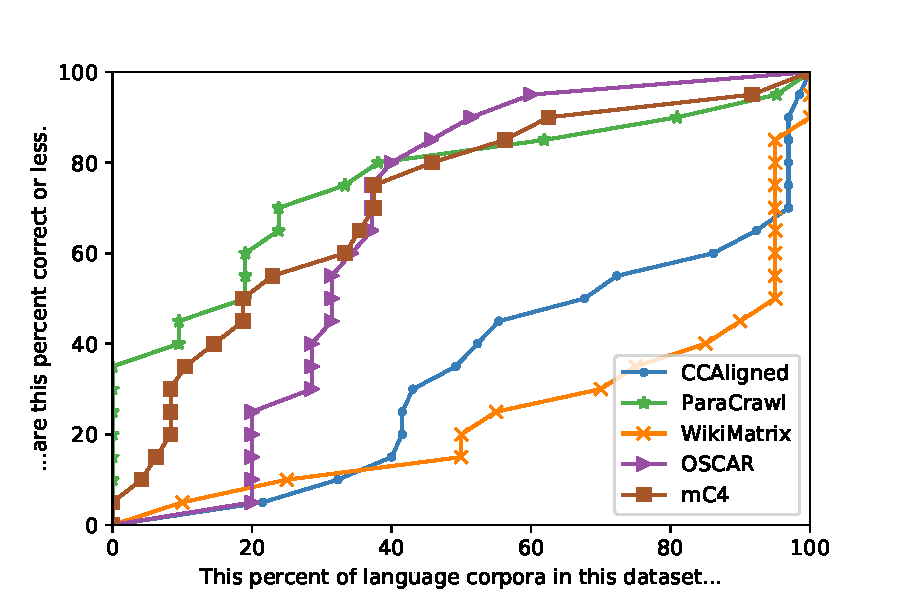
\includegraphics[width=\columnwidth]{static/media/oscar/quality/num_C_ratio.pdf}
    \caption{Fraction of languages in each dataset below a given quality threshold (percent correct).}% The larger the AUC, the better.}
    \label{fig:ratio_c}
\end{figure}

\paragraph{Why haven't these problems been reported before?}
The findings above are averaged on a per-language basis (i.e. macro-average), and therefore give low and high-resource languages equal weight. If we instead estimate the quality on a per-sentence basis, i.e. down-weight lower-resource languages in the computation of the average, the numbers paint a more optimistic picture (``micro'' block in Table~\ref{tab:results}). This is especially relevant for the monolingual datasets because they contain audits for English, which makes up for 43\% of all sentences in OSCAR 2019 and 36\% in mC4. To illustrate the effect of this imbalance: A random sample from the entire mC4 dataset with over 63\% chance will be from one of the 8 largest languages (\texttt{en}, \texttt{ru}, \texttt{es}, \texttt{de}, \texttt{fr}, \texttt{it}, \texttt{pt}, \texttt{pl}, $>$100M sentences each), %\footnote{mC4 contains 22\% \texttt{und} sentences, i.e. sentences with undefined language.} 
of which all have near perfect quality. Analogously, evaluation and tuning of web mining pipelines and resulting corpora in downstream applications focused largely on higher-resource languages (Section~\ref{sec:crawls}), so the low quality of underrepresented languages might go unnoticed if there is no dedicated evaluation, or no proficient speakers are involved in the curation~\citep{nekoto-etal-2020-participatory}.


\paragraph{How much content is nonlinguistic or in the wrong language?}
Nonlinguistic content is a more common problem than wrong-language content. Among the parallel datasets, CCAligned contains the highest percentage of nonlinguistic content, at 31.42\% on average across all rated corpora, and also the highest percent of wrong-language content, at 9.44\%. Among the monolingual datasets, mC4 contains the highest ratio both of sentences in incorrect languages (15.98\% average) and nonlinguistic content (11.40\% average), with 4 of the 48 audited languages having more than 50\% contents in other languages. The low amount of wrong language in ParaCrawl shows the benefits of selecting domains by the amount in-language text, but the dataset also covers the smallest amount of languages. The low ratio of wrong language samples in OSCAR may reflect the success of line-level LangID filtering.
These numbers provide evidence that more research in LangID could improve the overall quality, especially with respect to nonlinguistic content.

\paragraph{Which languages got confused?} The languages that were confused were frequently related higher-resource languages. However, there were also a significant number of ``out-of-model cousin" cases, where languages not supported by the LangID model ended up in a similar-seeming language. For instance in mC4, much of the Shona (\texttt{sn}, Bantu language spoken in Zimbabwe and Mozambique) corpus is actually Kinyarwanda (\texttt{rw}, Bantu language spoken in mostly in Rwanda and Uganda)---and, peculiarly, much of the Hawaiian (\texttt{haw}, Polynesian language spoken in Hawaii) is actually Twi (\texttt{tw}/\texttt{ak}, Central Tano language spoken mostly in Ghana).

\begin{figure}[th]
    \centering
    \begin{subfigure}{.5\textwidth}
        \centering
        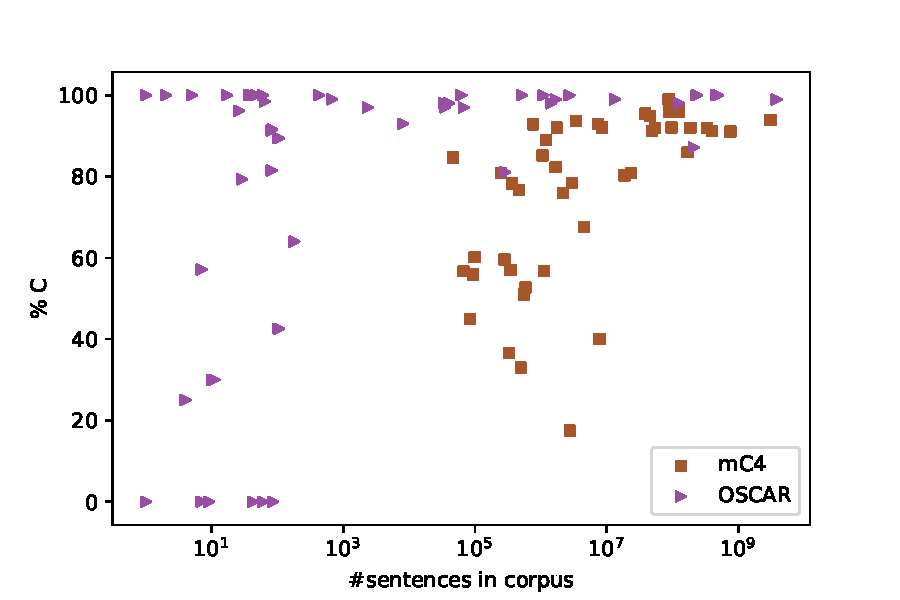
\includegraphics[width=\linewidth]{static/media/oscar/quality/C_mono.pdf}
        \caption{Monolingual corpora}
        \label{fig:C_mono}
    \end{subfigure}%
    \begin{subfigure}{.5\textwidth}
        \centering
        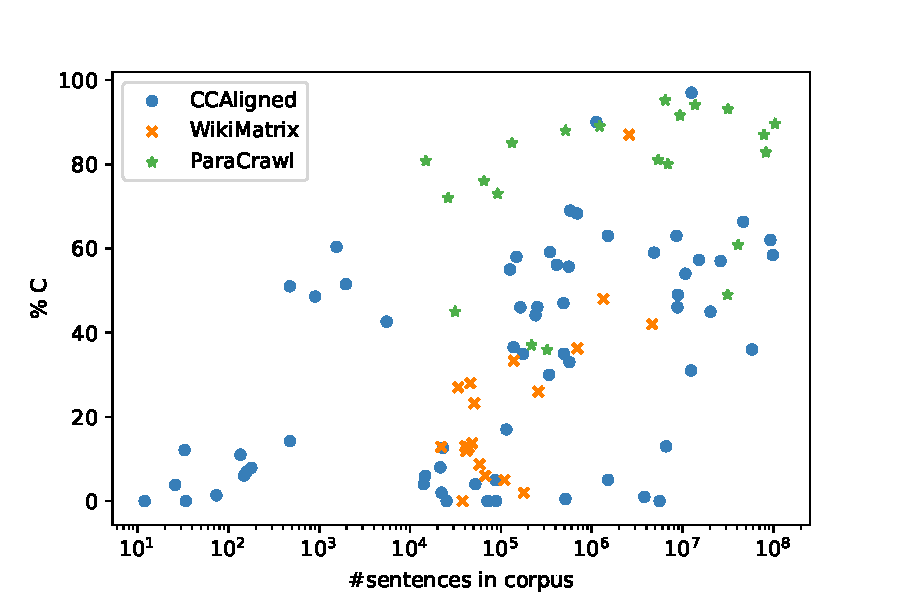
\includegraphics[width=\linewidth]{static/media/oscar/quality/C_para.pdf}
        \caption{Parallel corpora}
        \label{fig:C_para}
    \end{subfigure}
    \caption{Percentage of sentences labeled as correct vs. log N sentences for all audited languages.}
    \label{fig:C}
\end{figure}

\paragraph{Do low-resource languages have lower quality?}
Low-resource datasets tend to have lower human-judged quality.
The Spearman rank correlation between quality (\%\texttt{C}) and size is positive in all cases. The trend is strongest for mC4 ($r=0.66$), %,p=6.8e-8$), 
and gradually declines for CCAligned ($r=0.53$), %,p=0.0001$),
WikiMatrix ($r=0.49$), %,p=0.03$), 
ParaCrawl ($r=0.43$), %,p=0.02$) 
and OSCAR ($r=0.37$). %,p=0.10$).
Figure~\ref{fig:C} compares the number of sentences for each language against the proportion of correct sentences: %that we found during the audit:
%The correlation between quality (\%\texttt{C}) and size is strongest for WikiMatrix (Pearson's $r=0.66$), while mC4, CCAligned, ParaCrawl have comparatively lower correlation (0.21, 0.25, 0.29), and OSCAR the lowest with $r=0.13$.
%In general, we observe that languages with low representation tend to contain fewer correct sentences, with an exception of a dozen of languages from OSCAR.
Not all higher-resource languages ($>10^6$ sentences) have high quality, in particular for CCAligned (e.g. Javanese (\texttt{en\nobreakdash-jv\_ID}) with 5\%\texttt{C}, or Tagalog (\texttt{en\nobreakdash-tl\_XX}) with 13\%\texttt{C}). For mid-resource languages ($10^4$\nobreakdash--$10^6$ sentences) the picture is inconclusive, with some languages having high quality, and others having extremely low quality, even within the same datasets, e.g. Urdu in CCAligned \texttt{en-ur\_PK} has 100\%\texttt{C} vs. its romanized counterpart \texttt{en\nobreakdash-ur\_PK\_rom} 0.5\% \texttt{C}.
%\footnote{\texttt{\_rom} corpora have been removed in the latest CCAligned release.}
For individual error codes trends are less clear (not depicted).

\paragraph{Which languages have the lowest quality?} Across datasets we observe that the quality is particularly poor for languages that are included in romanized script (\texttt{\_rom}/\texttt{\_latn}), but are more commonly written in other scripts, e.g., Urdu (\texttt{ur}), Japanese (\texttt{ja}), Arabic (\texttt{ar}).
%\footnote{These romanized versions have been removed from CCAligned in a later release.} 
These are not transliterations of other scripts, but mostly contain non-linguistic material or wrong languages (e.g. the romanized Japanese corpus in mC4 (\texttt{ja\_latn}) contains Spanish, French, English, Portuguese, amongst others). %, Chinese (\texttt{zh}), Telugu (\texttt{te}) and Bulgarian (\texttt{bg}).  
In terms of geography, the poorest quality is found for African languages (Bambara (\texttt{bm}), Fula (\texttt{ff}), Kikongo (\texttt{kg}), Luganda (\texttt{lg}), Lingala (\texttt{ln}), Norther Sotho (\texttt{nso}), Oromo (\texttt{om}), Shona (\texttt{sn}), Somali (\texttt{so}), Tswana (\texttt{tn}), Wolof (\texttt{wo})), minority languages in Europe and the Middle East that are closely related to higher-resource languages (Azerbaijani (\texttt{az-IR}), North Frisian (\texttt{frr}), Neapolitan (\texttt{nap}), Silesian (\texttt{szl}), Zaza (\texttt{zza})), lesser spoken Chinese languages sharing a script with Mandarin (Yue (\texttt{yue}), Wu (\texttt{wuu})), four major Austronesian (Central Bikol (\texttt{bcl}), Chavacano (\texttt{cbk}), Javanese (\texttt{jv}), Sundanese (\texttt{su})), and some South-Asian languages, in particular Sinhala (\texttt{si}).
Appendix~\ref{app:stats} contains the detailed per-language statistics for all corpora.
% Omitted from above: mt

\paragraph{What is the incidence of offensive and pornographic content?}
Overall, the sampled sentences did not contain a large amount of offensive contents. However, there were notable amounts of pornographic content ($>10\%$) found in CCAligned for 11 languages. % not fully annotated: tl_XX, lt_LV ?

\begin{table}[!htbp]
    \centering
    \resizebox{\textwidth}{!}{%

        \begin{tabular}{lcccccccccccc}
            \toprule
                           & \texttt{es\_XX} & \texttt{bm\_ML} & \texttt{yo\_NG} & \texttt{tr\_TR} & \texttt{ku\_TR} & \texttt{zh\_CN} & \texttt{af\_ZA} & \texttt{jv\_ID} & \texttt{zh\_TW} & \texttt{it\_IT} & \textbf{mean} \\
            \midrule
            \textbf{Acc-6} & 0.58            & 0.73            & 0.41            & 0.45            & 0.43            & 0.55            & 0.65            & 0.55            & 0.46            & 0.55            & 0.66          \\
            \textbf{Acc-4} & 0.77            & 0.73            & 0.60            & 0.55            & 0.56            & 0.72            & 0.72            & 0.57            & 0.58            & 0.66            & 0.72          \\
            \textbf{Acc-2} & 0.91            & 0.96            & 0.72            & 0.64            & 0.71            & 0.79            & 0.77            & 0.92            & 0.81            & 0.69            & 0.79          \\
            \bottomrule
        \end{tabular}%
    }
    \caption{Rater evaluation for a subset of audits from \textbf{CCAligned} (translated from English) measured by the accuracy (Acc-$n$) of annotations by non-proficient speaker against annotations by proficient speakers.
        %$n$ indicates the granularity of the classes.  For $n=6$ all classes of the taxonomy were distinguished, for $n=4$ the \texttt{C} subclasses were combined, and for $n=2$ it is binary decision between \texttt{C} and the rest of the error classes.
    }
    \label{tab:agreement_ccaligned}
\end{table}

\begin{table}[!htbp]
    \centering\small

    \begin{tabular}{lccccccccc}
        \toprule
                       & \texttt{tyv} & \texttt{rm} & \texttt{bar} & \texttt{eml} & \texttt{zh} & \texttt{la} & \textbf{mean} \\
        \midrule
        \textbf{Acc-6} & 1.0          & 0.98        & 1.0          & 1.0          & 0.86        & 1.0         & 0.98          \\
        \textbf{Acc-4} & 1.0          & 1.0         & 1.0          & 1.0          & 0.87        & 1.0         & 0.98          \\
        \textbf{Acc-2} & 1.0          & 1.0         & 1.0          & 1.0          & 0.87        & 1.0         & 0.98          \\
        \bottomrule
    \end{tabular}%
    \caption{Rater evaluation for a subset of audits from \textbf{OSCAR 2019} measured by the accuracy (Acc-$n$) of annotations by non-proficient speaker against annotations by proficient speakers.}
    \label{tab:agreement_oscar}
\end{table}

\paragraph{Annotation quality}
For a subset of audited languages from CCAligned and OSCAR 2019 we measure the accuracy (Acc) of the labels assigned by non-proficient speakers against the labels assigned by proficient speakers for all audited sentences. This can be understood as a directed measure of annotator agreement for the special case where one rater is an expert and the other is not. Results for varying label granularity are reported in Tables~\ref{tab:agreement_ccaligned} and \ref{tab:agreement_oscar}. For $n=6$ all classes of the taxonomy were distinguished, for $n=4$ the \texttt{C} subclasses were combined, and for $n=2$ it is binary decision between \texttt{C} and the rest of the error classes. With the full 6-class taxonomy (Acc-6) we find a mean accuracy of 0.66
%($\sigma^2 =0.02$) 
for CCAligned audits, and 0.98
%($\sigma^2 =0.002$) 
for OSCAR audits. % (see appendix~\ref{app:agreement} for language-specific results).
With a binary taxonomy (Acc-2) distinguishing \texttt{C} from the rest, the accuracy further increases to 0.79
%($\sigma^2=0.01$) 
for CCAligned. This provides strong evidence that good quality annotations are not limited to those proficient in a language.

However, the significant drop of accuracy for finer-grained labels hints at that our taxonomy can be further improved, especially for parallel sentences.
The error taxonomy lacks at least one category of error, namely ``correct/in-language but unnatural".  Similarly, the definition of ``correct-short" and ``correct-boilerplate" were not understood equally by all annotators and the concept of ``correct-short" has potential issues for agglutinative languages like Turkish. Finally, it was unclear what to do with related dialects, e.g. when a sentence is ``almost correct but wrong dialect" or when it is unclear which dialect a sentence belongs to. We recommend including these categories for future audits

\subsection{Automatic Filtering}
Given the frequency of \texttt{WL} and \texttt{NL} annotations, it might be tempting to use open-source LangID models to post-filter data on a per-sentence(-pair) level, as OSCAR does. Unfortunately, this turns out to have its own issues.

\paragraph{Sentence-level n-gram LangID filtering}
We classify all sentence pairs of CCAligned with CLD3, an n-gram based LangID model. By comparing its predictions to the audit labels, we evaluate its quality on the subset of annotated samples: the classifier should detect both correct languages when the pair is annotated as \texttt{C} and \texttt{X}, and should detect incorrect languages in the pair when \texttt{WL} and \texttt{NL}. On this task, the CLD3 classifier
%\footnote{\texttt{filter=0.976 Prec, 0.962 Rec, 0.969 F1.}} 
achieves an average precision of only 40.6\%. %,
%n average accuracy of 56.4\% against our annotators across all audited sentences, 
%underlining the issues with LangID on web domain data~\citep{caswell-etal-2020-language}. %Its recall for detecting those pairs with wrong language(s) is 77.8\%, and its precision 35.9\%. 

\paragraph{Sentence-level Transformer LangID filtering}
N-gram LangID models like CLD3 have known problems. However, \citet{caswell-etal-2020-language} demonstrate that semi-supervised Transformer-based LangID models strongly out-perform them. We train a comparable Transformer-based LangID model and apply it to our annotated CCAligned data. We find that filtering noisy corpora ($<$ 50\% correct) on LangID for both source and target leads to gains in median precision, rising from 13.8\% pre-filter to 43.9\% post-filter. However, this comes at a steep cost of 77.5\% loss in recall.
The biggest winners were Lingala, whose precision climbs from 8\% to 80\%, and Oromo, which soars from 2\% to 33\% in-language. Both of these, however, come at the cost of losing 50\% of the correct in-language sentences, being reduced from ~22k sentences to 3k and 1k sentences respectively, which would likely be too small for building downstream models. The moral is that, at least at the current stage, there is no one-size-fits-all approach for sentence-level LangID filtering.


\section{Dataset Mis-labeling}
\label{sec:codes}
Standardized and unambiguous representations of language codes are important for practical data use and exchange. The standard used by most academic and industry applications is BCP-47~\citep{phillips-etal-2005-tags}, which builds off the two-letter ISO639-2 codes and three-letter ISO639\nobreakdash-3 codes, but also allows to add subtags for scripts (e.g. Hindi in Latin script: \texttt{hi-Latn}) or regional varieties (e.g. French spoken in Canada: \texttt{fr-CA}). It would enhance transparency and interoperability if adopted consistently, especially with growing language diversity in NLP.

We find a variety of errors and inconsistencies in language code usage, ranging from serious mislabelings to small transgressions against standard conventions. For this analysis, we also include the JW300~\citep{agic-vulic-2019-jw300} dataset, a multilingual dataset crawled from \url{jw.org}. %, which was otherwise not audited in this paper. 
In summary, we find 8 nonstandard codes in CCAligned, 3 in OSCAR 2019, 1 in mC4, 1 in WikiMatrix, and 70 in JW300, for 83 in total. This does not include the 59 codes affected by superset issues. %0 in ParaCrawl, 
Full details are given in Appendix~\ref{app:jw300}.

\paragraph{Inconsistent Language Codes} One common issue is simply using nonstandard or invented codes. For example, CCAligned uses only two-letter codes, so when the BCP-47 code for a language is three letters it is either shortened (e.g. \texttt{zza} $\rightarrow$ \texttt{zz}) or invented (\texttt{shn}  $\rightarrow$ \texttt{qa}). Similarly, OSCAR 2019 contains data labeled as \texttt{als} (BCP-47 for Tosk Albanian) that is actually in \texttt{gsw} (Allemannic).\footnote{This is a result of the language code used by the \href{https://en.wikipedia.org/wiki/Alemannic\_Wikipedia}{Alemannic Wikipedia} and affects any corpus or tool that uses Wikipedia data without correcting for this, like FastText.} 22 additional language codes in JW300 have similar issues, including 12 codes that start with \texttt{jw\_} but are not Javanese.

\paragraph{False Sign Languages}
12\% (48/417) of JW300
%has a much stranger problem than nonstandard codes. It has the peculiar issue that a full 12\% (48/417) of the languages it claims to cover 
carry language codes for sign languages. %While it is possible to transcribe sign languages using glosses, this is not what these corpora are. 
Instead of sign language transcripts they are texts in another high resource language, mostly English or Spanish---for example, the \texttt{en-zsl} (Zambian sign language) data is actually English-English parallel data (copies), details in Appendix~\ref{app:jw300}. This was likely caused by videos with sign language interpretation embedded on the crawled websites.\footnote{Kudos to Rebecca Knowles for this explanation.} %Details are in Appendix Table~\ref{tab:signlanguages}.


\paragraph{Mysterious supersets}
When datasets contain language codes that are supersets of other language codes, it is difficult to determine which particular language the text contains. WikiMatrix has Serbian (\texttt{sr}), Croatian (\texttt{hr}), Bosnian (\texttt{bs}), and Serbo-Croatian (\texttt{sh})---their superset.\footnote{\url{https://iso639-3.sil.org/code/hbs}}
%. And while there may be some debate whether \texttt{bs},  \texttt{hr},  \texttt{cnr},  and \texttt{sr} are different languages, \texttt{sh} (\texttt{hbs}) is by definition a superset of all of them.\footnote{https://iso639-3.sil.org/code/hbs} 
The issue of codes that are supersets of others is common enough to include a small table dedicated to it (Appendix Table~\ref{tab:supersets}).
In some cases this may not be an issue, as with Arabic, where \texttt{ar} conventionally refers to Modern Standard Arabic, even though the code technically encompasses all dialects.
%, or where \texttt{no} typically refers to Norwegian Bokm\r{a}l (\texttt{nb}), though it technically is the superset of \texttt{nb} and \texttt{nn}. 
In many cases, the nature of the data in the superset code remains a mystery.
% requiring detective work.


\paragraph{Deprecated codes} Finally, there are several deprecated codes that are used: \texttt{sh} in Wikimatrix, \texttt{iw} in mC4, \texttt{sh} and \texttt{eml} in OSCAR 2019, and \texttt{daf} in JW300.

\section{Risks of Low-Quality Data}\label{sec:risk}

\paragraph{Low quality in downstream applications}
Text corpora today are building blocks for many downstream NLP applications like question answering and text summarization---for instance, a common approach is to first train translation models on such data and then automatically translate training data for downstream models~\citep{conneau-etal-2018-xnli}. If the data used for the original systems is flawed, derived technology may fail for those languages far down the line without knowing the causes.
This risk of undesired downstream effects calls for future studies with a careful treatment of intertwined effects such as data size and domain, language-specific phenomena, evaluation data and metric biases.
%Furthermore, there are not many existing public models trained on these specific subsets of data that we can analyze. 
To give the reader a brief glimpse of the impact of data quality for the example of translation, we compare the \texttt{C}\% metric from our audit with the translation quality (sentencepiece-BLEU, spBLEU) of the multilingual translation model M2M124 for 124 languages~\citep{goyal-etal-2021-flores-101}. It was trained on WikiMatrix and CCAligned, and similar data collected with the same tools, which we expect to show similar biases. Translation quality is evaluated on the trusted, human-translated FloReS benchmark~\citep{goyal-etal-2021-flores-101}.
%For language pairs that were both covered in the WikiMatrix and the CCAligned audit, we compute an average of their \% \texttt{C} scores weighted by their size. 
For the 21 languages present in both the audit and the FloReS benchmark, we found a positive correlation (Spearman) between the data quality scores and spBLEU of $\rho=0.44$ $(p=0.041)$. This is not as large as the correlation with data size ($\rho=0.66$, $p=0.00078$), but it nonetheless helps to explain translation quality---the correlation between the product of \texttt{C}\% and data size (in other words, the expected total number of good sentences in the dataset), is the highest yet, with a value of $\rho=0.73$ $(p=0.00013)$.\footnote{For the translation from English, BLEU scores are less comparable but the trend holds nonetheless, with values of ($\rho=0.32$, $p=0.14$), ($\rho=0.74$, $p=0.000078$), and ($\rho=0.80$, $p=0.0000087$) respectively.}
% The human inspection and auditing of e.g. trained vector representations to detect possible risks and misrepresentations of a subset of languages is arguably harder than manually inspecting a few samples as we did in this work.
% As our analysis has shown, low-resource languages are disproportionately affected by such problems in automatic data curation pipelines.

\paragraph{Representation washing}
Since there are datasets which contain many low-resource languages, the community may feel a sense of progress and growing equity, despite the actual quality of the resources for these languages. %However, models often still perform poorly on NLP tasks for these languages
%Because there appear to be datasets for low-resource languages, the community may collectively feel as though progress is being made in these areas. 
Similarly, if low-quality datasets are used as benchmarks they may exaggerate model performance, making low-resource NLP appear more solved than it is---or conversely, if models perform poorly when trained with such data, it may be wrongly assumed that the task of learning models for these languages is harder than it actually is or infeasible given current resources. These effects could result in productive effort being redirected away from these tasks and languages.
%The result can be that productive effort will be directed away from these fields.

\begin{table}[t!]

    \centering\small
    \begin{tabular}{ll}
        \toprule

        \texttt{en}  & The prime minister of the \textbf{UK} is \textbf{Boris Johnson}.          \\
        \texttt{nl}  & De minister-president van \textbf{Nederland} is \textbf{Mark Rutte}.      \\
                     & \small{\texttt{en}: The prime minister of the Netherlands is Mark Rutte.} \\
        \midrule
        %\midrule
        % \texttt{en} &Sunglasses \\
        % \texttt{ig}	&ah\d{i}a Nyocha \\
        % \midrule
        \texttt{en}  & \textbf{24 March} 2018                                                    \\
        \texttt{pt}  & \textbf{14 Novembro} 2018                                                 \\
                     & \small{\texttt{en}: 14 November 2018 }                                    \\
        %\midrule
        \midrule
        % \texttt{en} &The current local time in \textbf{Sarasota} is \textbf{89} minutes ahead of apparent solar time. \\
        % \texttt{nn}	&Den lokale tiden i \textbf{Miami} er \textbf{86} minutt f\o{o}re sann soltid. \\
        \texttt{en}  & The current local time in \textbf{Sarasota} is \textbf{89} minutes.       \\
        \texttt{nn}  & Den lokale tiden i \textbf{Miami} er \textbf{86} minutt.                  \\
                     & \small{\texttt{en}: The local time in Miami is 86 minutes.}               \\
        %\midrule
        \midrule
        \texttt{en}  & In \textbf{1932} the highway was extended \textbf{north to LA}.           \\
        \texttt{bar} & \textbf{1938} is de Autobahn bei \textbf{Inglstod} fertig gstellt.        \\
                     & \small{\texttt{en}: The highway near Inglstod was completed in 1938.}     \\
        % \midrule
        % \textit{en:} He was engaged to the lawyer and actor João Lima Junior, with whom he dated from 2004 to 2006. \\
        % \textit{nds:} Ze woont in de tussentied samen met zanger en liedtiesschriever Johannes Oerding met wie ze sinds 2009 ook samen op de bühne stiet.\\
        \bottomrule
    \end{tabular}%
    \caption{Examples of ``parallel" data where the translation has a different meaning than the source, but the form looks the same. (We added translations of the non-English side.) Such data may encourage hallucinations of fake ``facts".}
    \label{tab:not_actually_parallel}
\end{table}

\paragraph{Trust in incorrect ``facts''} % and trust} %, algorithmic trust and automation bias}
We found many instances of parallel-looking sentences that are structurally and semantically similar, but not factually correct translations (Table~\ref{tab:not_actually_parallel}). They can cause models to produce plausible ``translations" that are factually wrong, but users may still trust them (\textit{algorithmic trust}) without verifying the information. %This is relevant for \textit{algorithmic trust}, when users increasingly trust the outputs of computers and ``algorithms" without verifying the information. 
Similarly, \textit{automation bias} \citep{skitka-etal-1999-does},
%from social psychology which refers to the bias of 
referring to humans favoring decisions made by automated systems over decisions made by humans, might amplify the issues of inaccurate translations caused by misalignments.
%One variant of this issue that occurs frequently in some datasets is pornographic content.
%, which in the majority of the cases we observed were parts of misaligned sentence pairs. 
%Another effect is that models trained on misaligned pornographic content may hallucinate such content, which may be disturbing to users.

\section{Future Work and Recommendations}\label{sec:recommendation}
Of the five multilingual corpora evaluated, we consistently found severe issues with quality, especially in the lower-resource languages. We rated samples of 205 languages, and found that 87 of them had under 50\% usable data, with a full 15 languages at 0\% in-language. We furthermore found consistent issues with mislabeled data and nonstandard language codes, particularly in the JW300 dataset, and identified 83 affected corpora, at least 48 of which were entirely spurious (Section~\ref{sec:codes}). While there might have been anecdotal evidence of insufficient quality for some datasets, the majority of these quality issues had not been reported, nor been investigated in depth. These issues might go unnoticed for languages that are not represented in the evaluation of the crawling methods, and cause harm in downstream applications~\citep{khayrallah-koehn-2018-impact}.

There are a variety of ways to improve both the ease and accuracy of human evaluation, as well a few classes of issues we ignored in this paper, like close dialects.
Ideally we would like to build a standard suite of automatic metrics for datasets, but more research is necessary to determine what the appropriate metrics would be. One important area missing from our analyses however is the estimated portion of a dataset which has been generated by MT~\citep{rarrick-etal-2011-mt}, LM systems, or bots/templates, as for example in the analysis of C4~\citep{dodge-etal-2021-documenting}. %A prominent example is the Lsjbot\footnote{\url{https://en.wikipedia.org/wiki/Lsjbot}} which is responsible for creating 80-90\% of content for Swedish, Cebuano and Waray Wikipedia. 
The information captured in machine-generated content might still be useful for modeling, but might falsely overrepresent typical generation patterns and introduce linguistic errors or unnatural artifacts.
% Malagasy wiktionary audit: https://meta.wikimedia.org/wiki/Requests_for_comment/Large-scale_errors_at_Malagasy_Wiktionary
%https://www.vice.com/en/article/4agamm/the-worlds-second-largest-wikipedia-is-written-almost-entirely-by-one-bot

% Finally, similar studies to this in future would do well ton work more on calibrating human raters, to ensure consistent use of error categories.

% An issue that arises with the progress in building technology for some of the languages is the retrieval of machine-generated output as in-language data. This is prominent for mid- to high-resource languages for which translation systems have reached sufficient quality for website translation, as we observed for example a significant amount of translations for Ukrainian. Non-native speakers might not have noticed them during annotations, so the problem might be even larger than we might estimate now. We leave a systematic investigation to future work. A more unexpected artifact is the retrieval of published BPE vocabularies for a range of low-resource languages, such as Sundanese.\footnote{\url{https://nlp.h-its.org/bpemb/su/su.wiki.bpe.vs100000.vocab}

We therefore strongly recommend looking at samples of any dataset before using it or releasing it to the public. As we have shown, one does not need to be proficient in a language to see when there are serious quality issues, and a quick scan of 100 sentences can be sufficient to detect major problems. Moreover, going through and annotating a small sample of data can bring actionable insights about new ways to filter or use it.

If data quality issues are found, a wide variety of techniques can be explored, like filtering on length-ratio, LangID, TF-IDF wordlists \cite{caswell-etal-2020-language} or dictionaries~\citep{kamholz-etal-2014-panlex}; to neural approaches like LM scoring \cite{axelrod-etal-2011-domain,moore-lewis-2010-intelligent,wang-etal-2018-denoising}. Unfortunately, none of these provides a quick and easy fix, especially for low-resource languages---data cleaning is no trivial task!

Noisy datasets are by no means useless, at least if they contain some desirable content. Therefore, an alternative to filtering can be documentation~\citep{bender-etal-2021-on}. This can take the form of a per-language quality score and notes about known issues,
% ({ \it``language xx has high percentage non-linguistic content'' } etc.), 
a datasheet \citep{gebru-etal-2018-datasheets} or nutrition label \citep{holland-etal-2018-the}. However, we suggest researchers not release corpora with near-zero in-language content, as this may give the mistaken impression of usable resources.

Finally, we encourage the community to continue conducting evaluations and audits of public datasets---similar to system comparison papers.

\section{Conclusions for the OSCAR Project}

While the study described in chapter \ref{chap:monolingual} showed encouraging results for the OSCAR 2019 corpus, a lot of concerns about the actual quality of the data remained unaddressed. This has addressed some of these concerns and actually showed promising results for the OSCAR corpus especially in comparison to the other four audited corpora, as OSCAR 2019 obtained the highest percentage of correct sentences as shown in table \ref{tab:results}.

However, we also acknowledge that major issues remain to be addressed as has been pointed out here and more importantly, only $0.00004\%$ of the corpus was actually audited here, meaning that potential issues with both the corpus and the pipeline might remain to be discovered. This collaboration marks thus a turning point for the OSCAR project, as it served as a platform and catalyst for both relaunching the project and start working on further versions of the corpus to the one originally published in 2019 \citep{ortiz-suarez-etal-2019-asynchronous}. The following two chapters will describe the creation of two subsequent versions of OSCAR that try to address some of the problems described here and some others that were pointed by the users of the project at both the corpus and the pipeline level.

